\begin{exo}
	Lorsque le basketteur Stephen Curry tire en match, il y a $53$\% de chance que ce soit un tir à $2$ points et $47$\% que ce soit un tir à $3$ points.

	De plus, quand il tire à $2$ points, son pourcentage de réussite est de $51,5$\% contre $43,5$\% à $3$ points.

	Lorsque Curry tire en match, on considère les événements :

	\begin{itemize}
		\item $D$ : \og{} Il tire à $2$ points \fg{}
		\item $M$ : \og{} Il marque. \fg{}
	\end{itemize}

	\begin{enumerate}
		\item Compléter l'arbre pondéré ci-dessous :
	\end{enumerate}

	\begin{center}
		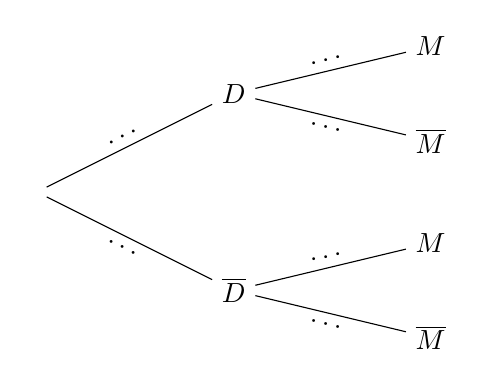
\begin{tikzpicture}[grow=right, sloped, level distance=2.5cm,
				level 1/.style={sibling distance=2.5cm},
				level 2/.style={sibling distance=1.2cm}]

			\node {}
			child {node {$\overline{D}$}
					child {node {$\overline{M}$} edge from parent node[below] {\dots}}
					child {node {$M$} edge from parent node[above] {\dots}}
					edge from parent node[below] {\dots}
				}
			child {node {$D$}
					child {node {$\overline{M}$} edge from parent node[below] {\dots}}
					child {node {$M$} edge from parent node[above] {\dots}}
					edge from parent node[above] {\dots}
				};
		\end{tikzpicture}
	\end{center}
	
	\begin{enumerate}[resume]
		\item Calculer la probabilité que Stephen Curry tente un tir à $2$ points et le marque.
		\item Calculer la probabilité $P\pa{\overline{D} \cap M}$ et interpréter cette valeur dans le contexte de l'exercice.
	\end{enumerate}

	On admet que :
	\[
		P\pa{M} = P\pa{D \cap M} + P\pa{\overline{D} \cap M}
	\]

	\begin{enumerate}[resume]
		\item Calculer la probabilité $P\pa{M}$ qu'il marque son tir.
	\end{enumerate}
\end{exo}
